%%=============================================================================
%% Methodologie
%%=============================================================================

\chapter{Methodologie}
\label{ch:methodologie}

%% TODO: Hoe ben je te werk gegaan? Verdeel je onderzoek in grote fasen, en
%% licht in elke fase toe welke stappen je gevolgd hebt. Verantwoord waarom je
%% op deze manier te werk gegaan bent. Je moet kunnen aantonen dat je de best
%% mogelijke manier toegepast hebt om een antwoord te vinden op de
%% onderzoeksvraag.

\section{Wat zijn de redenen van een omschakeling?}
\label{sec:methodologie-redenen-omschakeling}

TO DO

- slechte monitoring
- slecht geautomatiseert 
- geen multi environment
- expert vertrokken
- gui veel werk en complex
- oorspronkelijk geen modules, refactor, in feite nu weer refactor
- updates zorgen voor compatiblieteistproblemen (denk ik)
- puppet client niet ouder dan puppet master maar omgekeerd denkik wel (op te zoeken)

\section{Technische werking van Ansible en Puppet?}
\label{sec:methodologie-technische-verschillen}

\subsection{Overzicht van Puppet en Ansible}



\begin{minipage}{15cm}
\begin{tabular}{ r |c c }
& \textbf{Ansible} & \textbf{Puppet} \\
  \hline	  		
\gls{deploytijd}  & declaratief & declaratief  \\
   \hline
 Programmeertaal & YAML & eigen \gls{dsl}  \\
     \hline
   Communicatieprotocol & SSH & HTTPS \\
   \hline
  Push / Pull principe (standaard)\footnote{Beide technologie\"en zijn in staat om zowel volgens push als pull methode te functioneren. Zo heeft Ansible 'pull-mode' en Puppet 'Puppet kick' \autocite{ansiblepull]} \autocite{puppetkick}} & \gls{push} & \gls{pull} \\
   \hline
   open poorten\footnote{Dit zijn de minimale vereisten van open poorten. Voor sommige features dienen meer poorten open te staan. Bijvoorbeeld 443 voor Ansible Tower of 8140 op elke Puppetclient voor de Puppet kick functionaliteit \autocite{puppetkick} }  & 22/tcp (client) & 8140/tcp (master)\\
  \end{tabular}
  \end{minipage}   



 \textcite{languagePuppet}, \textcite{masterproef}, \textcite{ansibledoc}

\subsection{Werking van Puppet}

Tussen de master en de client bestaat er een vertrouwensrelatie die onderhouden wordt door certificaten. Het is de Puppetmaster die verantwoordelijk is voor het verlenen van deze certificaten. Pas als deze in orde zijn kan Puppet  aan de configuraties van de clients beginnen. De verzameling van alle geschreven code wordt een manifest genoemd. Wanneer een Puppetagent wil controleren of hij nog up-to-date is, zal hij een catalogus aanvragen bij de Puppetmaster. Een dergelijke catalogus is in feite een manifest dat de Puppetmaster compileert. Deze catalogus is bovendien uniek voor elke Puppetagent. Dit komt omdat er bij het compileren van het manifest naar de catalogus rekening gehouden wordt met diverse parameters zoals de functie van de server of de distributie van het besturingssysteem dat op die server draait \autocite{Puppetlanguagecatalog}. Eens de Puppetagent zijn persoonlijke catalogus ontvangen heeft, zal deze voor zichzelf controleren of er verschillen zijn tussen zijn huidige configuratie en de staat die beschreven staat in de catalogus. Indien er afwijkingen zijn, worden deze ook automatisch opgelost \autocite{puppetdoc}.

\begin{figure}  \begin{center}
  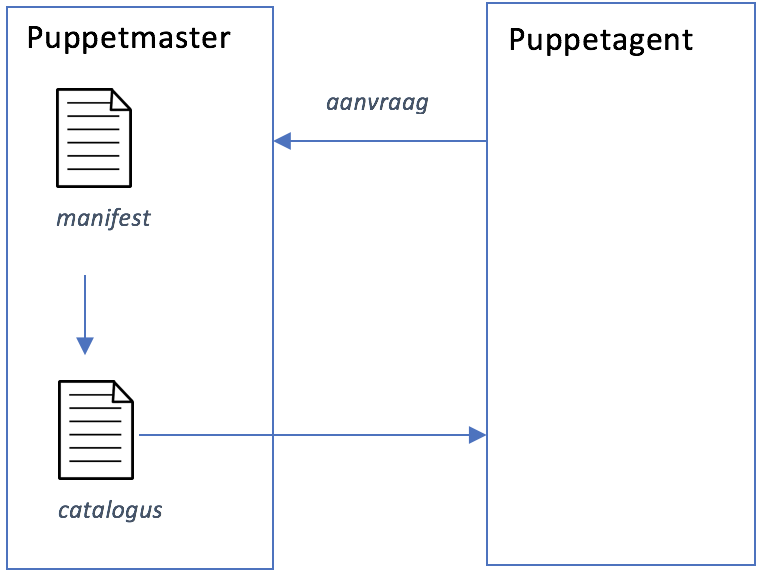
\includegraphics[width=250px]{img/aanvraagCatalogus.png}
 \end{center}\caption{aanvraag van een catalogus bij de Puppetmaster door een Puppetclient. De Puppetagent is een deamon (stukje software) die op de Puppetclient draait.}  
  \label{fig:aanvraagCatalogus}
\end{figure}


\subsection{Werking van Ansible}

In tegenstelling tot Puppet maakt Ansible geen gebruik agents. Dit betekent dat de Ansibleserver enkel de naam en het wachtwoord dient te kennen van de servers die hij moet configureren. Het authenticeren kan op verschillende manieren. Er wordt aangeraden om gebruik te maken van een SSH-key, wat het eenvoudigst is, maar ook andere middelen zoals een eenvoudig wachtwoord of het Kerberos-protocol worden ondersteund. De gewenste configuraties worden geschreven in playbooks met bijhorende modules. Eens een verbinding tot stand is gebracht, wordt dit playbook met zijn modules verstuurd naar de te configureren server. Deze worden vervolgens op de Ansible clients uitgevoerd  en weer verwijderd. Ook Ansible bezit de functionaliteit om na te gaan of de huidige configuratie in lijn is met de ontvangen modules. Om servers te configureren met Ansible bestaan er bovendien twee manieren. Ansible playbooks kunnen in principe verstuurd worden naar de servers vanaf elke computer. Voor een grotere hoeveelheid servers is dit echter moeilijk onderhoudbaar en onoverzichtelijk. Hiervoor bestaat er de commerci\"ele versie waarbij de playbooks worden verstuurd vanaf een centraal punt. Dit centraal punt is voorzien van Ansible Tower die een inventaris heeft van alle servers en playbooks die onder zijn verantwoordelijkheid vallen. Verschillende gebruikers kunnen vervolgens verschillende toegangsrechten krijgen zodat personen enkel servers kunnen configureren die onder hun bevoegdheid vallen \autocite{ansibledoc}.

%------------------------------------

\section{Technische analyse van Ansible en Puppet?}
\label{sec:technischeanalyse}
\subsection{Opstelling van de test omgeving}
\label{sec:opstellingtestevn}
\subsubsection{Architectuur van de opstelling}

\begin{wrapfigure}{R}{0.3\textwidth}
\centering
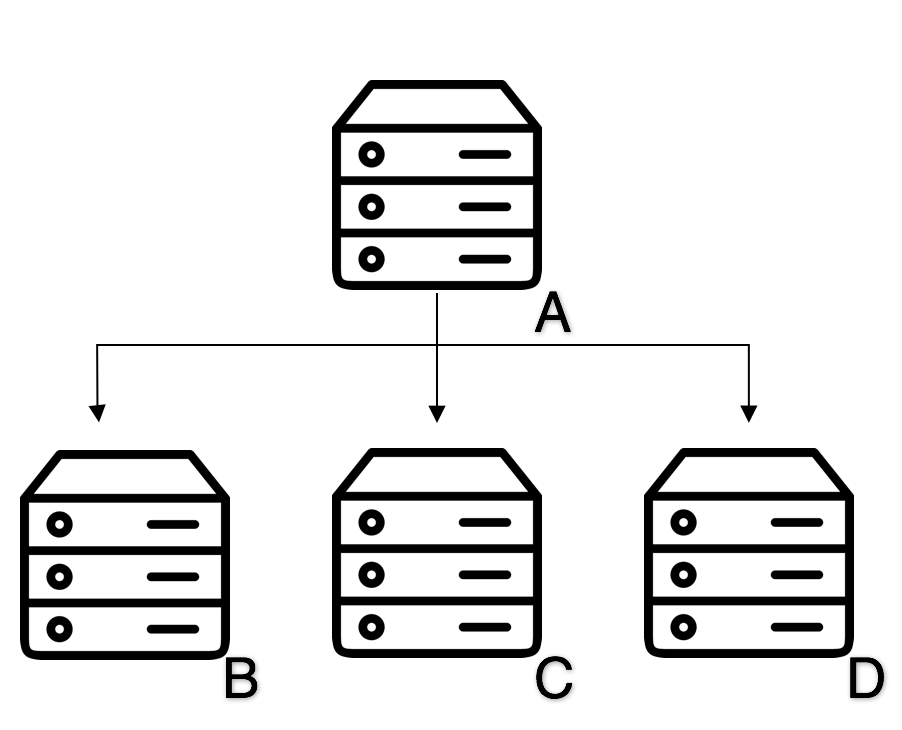
\includegraphics[width=0.25\textwidth]{img/infrastructruur.png}
\caption{\label{fig:infrastructuur} Server A, de master, configureert server B - D, de clients.}
\end{wrapfigure}


Deze opstelling is gerealiseerd door gebruik te maken van twee Vagrant bestanden. Voor elk Vagrant bestand word eerst de master aangemaakt, gevolgd door X aantal client's. Vagrant zorgt ervoor dat elke client  verbonden wordt met New Relic, de gekozen tool om de servers te monitoren. In het geval van Puppet wordt hierbij ook nog de Puppet agent ge\"installeerd. Elke client, zowel in de Ansible- als de Puppetinfrastructuur, is gebaseerd op dezelfde basebox en krijgen dezelfde resources toegekend. De masters beschikten over meer resources.\newline

\fbox{\begin{minipage}{15em}
\textbf{Technische specificaties clients}\newline
Basebox: bertvv/centos72\newline
Aantal CPU's: 1\newline
Geheugen: 500 MB
\end{minipage}}

\subsubsection{Configuraties van de deploy's}


Voor de testen in sectie \ref{sec:technischeanalyse} is er gekozen om gebruik te maken van een LAMP-stack. Dit is zowel voor Ansible als Puppet gebeurt. Bovendien is er getracht geweest om in de mate van het mogelijke beide configuraties zo analoog mogelijk te houden. Om dit te realiseren wordt er httpd, php, php-mysql en mariaDB-server ge\"installeerd. Vervolgens wordt er een webpagina op de site geplaatst. Deze is geschreven in PHP en controleert of alle zaken werken naar behoren. Om af te sluiten wordt HTTP doorgelaten door de firewall, de service httpd gestart en MariaDB gestopt. \newline

Opmerking: De reden dat MariaDB op dit moment niet gestart wordt is vanwege de \gls{partialconfig}. Hierbij wordt gekeken hoelang het duurt om bij een bestaande configuratie enkele aanpassingen door te voeren. Het is dus pas hier dat MariaDB gestart wordt.



 
\subsection{Performantie}

Het is interessant om te weten wat de verhouding is tussen de gemiddelde deploytijd van Ansible en Puppet. Om dit op een zo betrouwbaar mogelijke manier te kunnen verwezenlijken, zijn de configuraties van Ansible en Puppet zo analoog mogelijk gehouden zoals te lezen was in sectie \ref{sec:opstellingtestevn}. Vervolgens wordt elke configuratie 30 keer uitgevoerd. De tijd kan worden onderverdeeld in twee delen.\newline
Het eerste deel van de tijd zal de \gls{connectietijd} genoemd worden. Dit is de tijd die het kost alvorens er effectief overgegaan kan worden tot configureren. Hieronder zitten zaken zoals het opstellen van een verbinding, het verzamelen van nodige gegevens en het versturen van een gepersonaliseerde configuratie. Bij Ansible kon deze tijd gewoon berekend worden op basis van de resultaten\footnote{connectietijd = totaal verstreken tijd -  \unexpanded{$ \sum  $} (tijd playbooks)}. Bij Puppet is dit echter niet mogelijk en bijgevolg zijn deze resultaten met de hand gemeten.\newline
 De tweede tijd is de \gls{deploytijd}. Dit is de tijd die nodig is om de configuratie effectief uit te voeren. Beide waarden zijn gebaseerd op de feedback van de corresponderende \gls{CMT}.




\subsubsection{\gls{deploytijd}}
\begin{figure}
  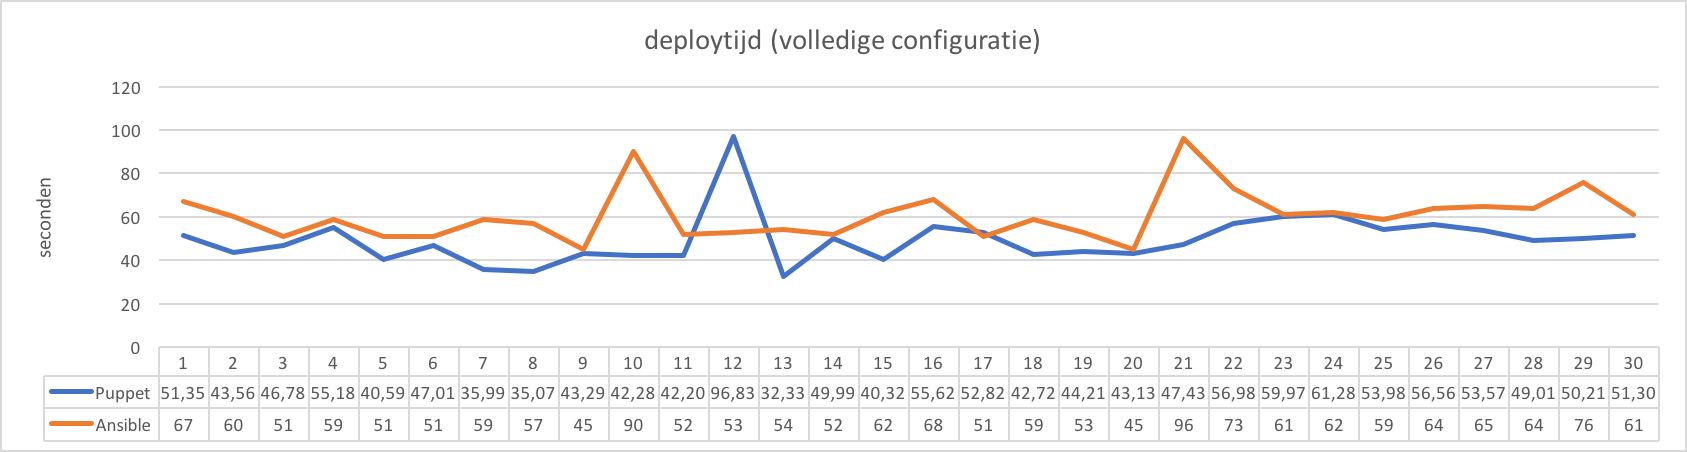
\includegraphics[width=\linewidth]{img/deploytime_fullconfig.png} 
  \caption{Tijd tot het bekomen van een consistente staat, vertrekkende van een 'lege' server.}  
  \label{fig:deploytime_fullconfig}
\end{figure}

Aangezien grafiek \ref{fig:deploytime_fullconfig} geen duidelijk verschil toont tussen beide \gls{CMT}'s zal met behulp van de Z-toets aangetoond worden of er al dan niet een statistisch verschil is.

\ref{wis:hypothesedeploytijd}

\underline{Conclusie} \newline
Z valt buiten het kritisch gebied waardoor de nulhypotese verworpen kan worden. Bijgevolg wordt aangenomen dat beide gemiddelden niet tot dezelfde verzameling behoren. Er kan dus worden geconcludeerd dat wanneer er wordt vertrokken van een lege server, Ansible er gemiddeld langer over doet dan Puppet. Dit is in dit geval een verschil van 11,3 seconden. \newline

De verschillen worden echter nog groter wanneer de test gedaan wordt met een gedeeltelijke configuratie. Hiermee wordt bedoeld dat er is vertrokken van servers die reeds geconfigureerd zijn en slechts enkele aanpassingen moeten doorgevoerd worden. Deze aanpassingen zijn een service starten en de inhoud van de webpagina veranderen. De resultaten lopen niet door elkaar waardoor een Z-toets niet echt nodig is. Ansible deed gemiddeld 19,10 seconden voor de deploy met een vrij grote variatie van 33,40 seconden. Puppet haalde maar een vrij consistente 3,10 seconden met een variatie van 0,35. \newline

In laatste instantie is er gekeken naar de tijd die het zou kosten tot de \gls{CMT} vaststelt dat de server reeds volledig is geconfigureerd en dat geen aanpassingen nodig zijn. Hierbij resulteert Ansible op een gemiddelde van 18 seconden met opnieuw een vrij grote variatie van 18,25 seconden. Ook hier doet Puppet het opnieuw beter waarbij er minder dan een seconde nodig heeft om vast te stellen dan dat geen aanpassingen nodig zijn. Uiteraard zijn al deze waarden afhankelijk van de configuratie maar ze geven wel een duidelijke indicatie van de verschillen tussen beide \gls{CMT}'s.

\textbf{Opmerking:} De \gls{connectietijd} is niet meegerekend in deze metingen. Het omvat hier uitsluitend de \gls{deploytijd}.
\subsubsection{\gls{connectietijd}}
Ook hier lopen de resultaten door elkaar zoals te zien is op grafiek \ref{fig:connectiontime}, bovendien liggen de gemiddelden hier veel dichter bij elkaar. Om vast te stellen of er een significant verschil is, zal er opnieuw gebruik gemaakt worden van de Z toets.
\begin{figure}
  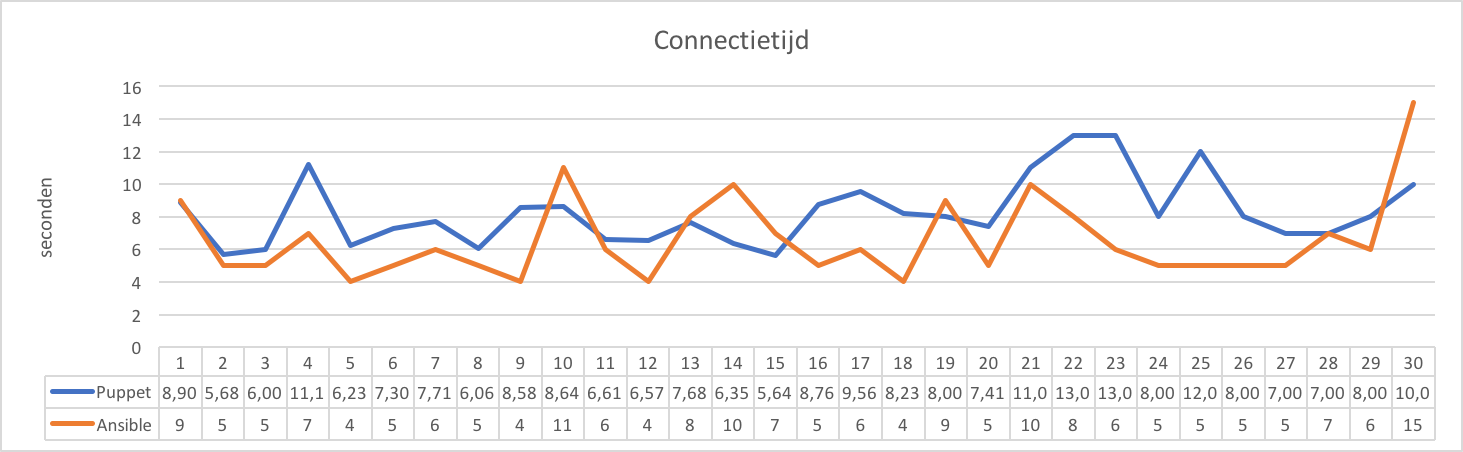
\includegraphics[width=\linewidth]{img/connectiontime.png} 
  \caption{Tijd tot het initialiseren van een deploy}  
  \label{fig:connectiontime}
\end{figure}



\ref{wis:hypotheseconnectietijd}

Z ligt in het aanvaardingsgebied waardoor we de nulhypothese, die stelt dat beide gemiddelden gelijk zijn, kunnen aanvaarden. Er is bijgevolg geen statistisch verschil tussen beide waarden.

%%---------------------------------------------------- einde performantie
\subsection{Belasting van het netwerk}

Ansible en Puppet hebben een groot verschil in de manier van communiceren en dit weerspiegelt zich in het gedrag van de \gls{CMT}. De grafieken op afbeeldingen \ref{fig:netwerkverbruik} en \ref{fig:deploytypes} weerspiegelen uitsluitend het dataverkeer tussen de server (Ansible Tower of Puppetmaster) en de desbetreffende client. Andere data, zoals bijvoorbeeld het downloaden van services of uploaden van logbestanden naar de monitoringstool, zijn hierin \underline{niet} opgenomen. Dit wordt verwezenlijkt door gebruik te maken van verschillende netwerkkaarten. Wanneer er geen deploy gebeurt, is de kilobyte/ minuut op deze netwerkkaart gelijk aan nul; een bewijs dat hier geen andere data dan deze van de \gls{CMT} over wordt verstuurd.  \newline

De manier van communicatie is te herkennen in de grafieken. Zo onderhoudt Ansible de communicatie met de client gedurende de deploy. Hiermee wordt bedoeld dat Ansible op de hoogte is van de laatste stand van zaken op de client. Wanneer een bepaalde taak voltooid is, wordt Ansibel Tower hier onmiddellijk van op de hoogte gebracht. Zoals te zien is op grafiek \ref{fig:deploytypes} is er geregeld communicatie tussen beide servers. Weliswaar is er enkel communicatie wanneer iets voltooid is; er is dus geen onnodige communicatie. Zo is ook te zien hoe op t6 de communicatie nul is. Ansible had voor die periode niets te melden\footnote{Hier betreft het de service MariaDB die werd ge\"installeerd}. \newline
 Deze manier van werken is handig tijdens het schrijven van nieuwe Ansible rollen. Je krijgt namelijk live feedback tijdens het uittesten. Een nadeel is wel dat het netwerk geen rust krijgt. Bovendien wordt deze functionaliteit van 'live feedback' in productie niet vaak gebruikt. In realiteit lopen deze jobs tijdens de nacht en is het voldoende om de dag daarna een algemeen overzicht te krijgen.\newline

Bij Puppet is dit anders. Hierbij is er enkel communicatie tussen de server en de client bij het begin en op einde van de deploy. Opmerkelijk hierbij is dat er twee types te herkennen zijn. Op figuur \ref{fig:deploytypes} zijn deze Puppet type A en B genoemd. Bij Puppet type A is te zien hoe de deploy bestaat uit twee reeksen terwijl dit bij type B uit drie reeksen bestaat. De oorzaak van deze derde reeks is niet gekend. Het opnieuw versturen van de tweede reeks was tijdelijk een piste maar dit is vermoedelijk niet het geval. Moest er een tcp-pakketje verloren gegaan zijn, zou uitsluitend dat pakketje opnieuw verstuurd worden en niet de hele reeks. Verder heeft de poging om de inhoud van de pakketjes te lezen tot niet veel geleid. De verbinding is namelijk ge\"encrypteerd door het HTTPS-protocol met als gevolg dat tools zoals Wireshark of tcpdump geen oplossing konden bieden over de inhoud hiervan.\newline
Een nadeel aan het feit dat er enkel in het begin en ophet einde communicatie is, is dat er op de master geen live feedback voor testen gevolgd kan worden. Dit kan echter wel opgelost worden door in te loggen op de client en hier de live feedback volgen met het commando "\texttt{puppet agent -t}". Het wordt wel nog steeds pas op het einde van de deploy terug naar de master gestuurd.
 \newline


Vervolgens is er ook gekeken naar de totale netwerkbelasting. Hiervoor is er per client een cumulatie genomen van de kilobytes/minuut gedurende de gehele deploy. Deze waarden zijn terug te vinden in grafiek \ref{fig:netwerkverbruik}. Hier heeft Ansible een gemiddelde van 5802,29 kilobytes/deploy. Puppet heeft bij deploy's van type A (bestaande uit twee reeksen) een gemiddelde van  9392,5 kilobytes/deploy en bij type B (bestaande uit drie reeksen) 13742,35 kilobytes/deploy. Gezamelijk heeft Puppet een gemiddelde van 11777,90 kilobytes/deploy. 


\begin{figure}
  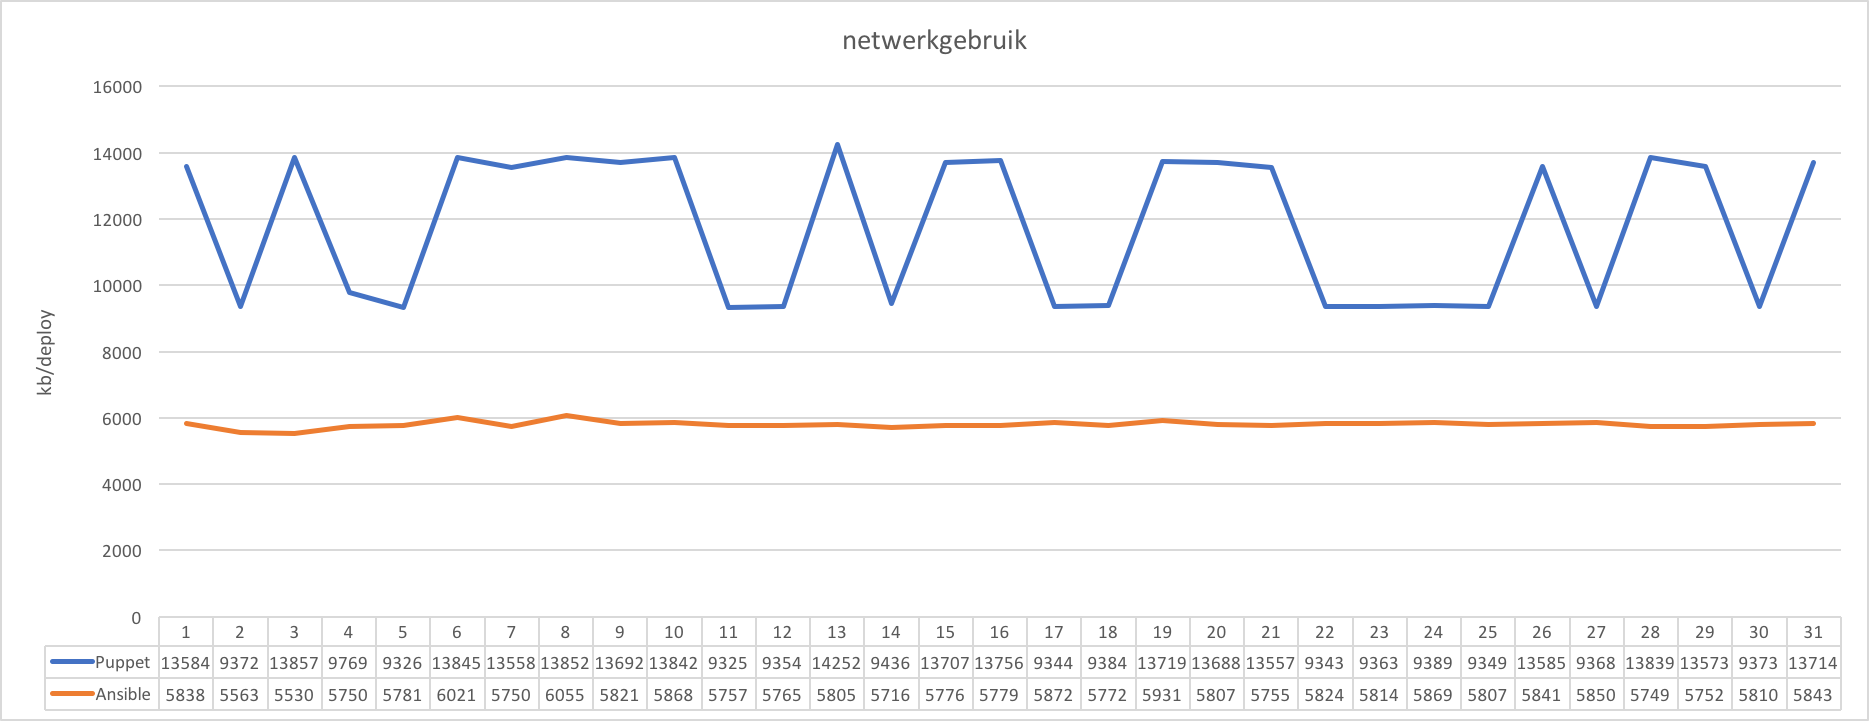
\includegraphics[width=\linewidth]{img/netwerkverbruik.png}
 \caption{Totaal verbruikte netwerkcapaciteit per client gedurende het deployen. Dit bevat enkel communicatie tussen master en client.}  
  \label{fig:netwerkverbruik}
\end{figure}


\begin{figure}
  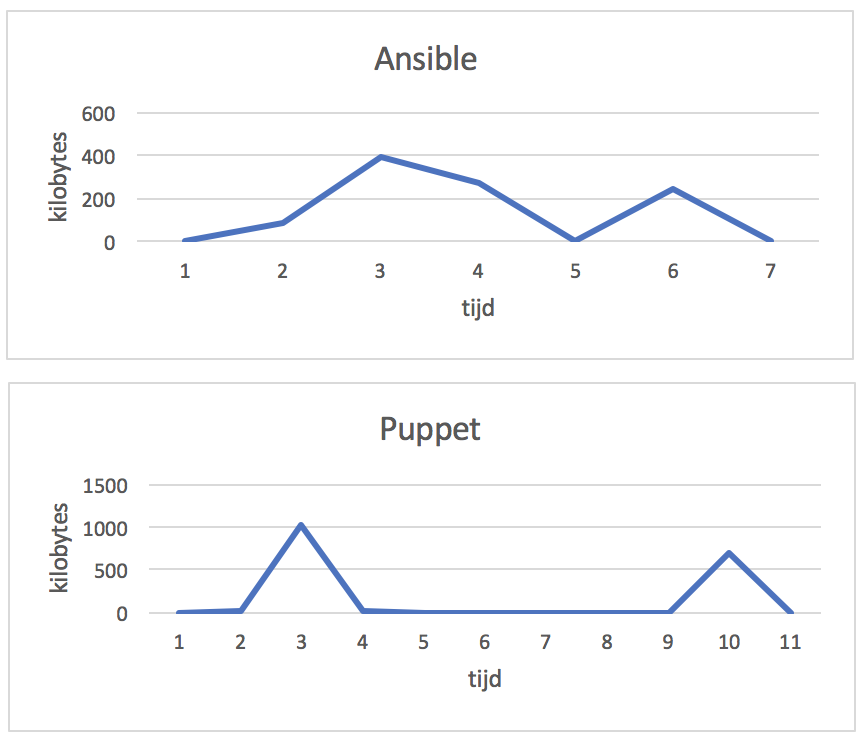
\includegraphics[width=\linewidth]{img/deploytypes.png}
 \caption{Drie types van communicatie. Aantal kilobytes per tijdseenheid op een netwerkkaart die uitsluitend bedoeld is voor communicatie met Ansible Tower / Puppetmaster. }  
  \label{fig:deploytypes}
\end{figure}

\subsection{Gebruik van het geheugen}

Op grafiek \ref{fig:geheugengebruik} is per tijdseenheid het gemiddeld gebruikt ramgeheugen weergegeven. Hierop is te zien hoe Puppet opvallend meer geheugen gebruikt. Niet alleen tijdens een deploy maar ook ervoor en erna. Zelfs wanneer een Ansible client en een Puppet client juist opgezet worden met behulp van de Vagrantfile, is er al een verschil in het gebruikte geheugen. Gezien het feit dat er al een verschil waar te nemen is in deze vroege levensfase van de server en het enige verschil in configuratie op dit moment de Puppetagent is, werd vermoed dat het verschil hier aan te wijten is. Dit vermoeden werd gestaafd toen de Puppetagent tijdelijk uitgezet werd. Het ramgeheugen daalde onmiddellijk naar gelijkwaardige waarden als deze van de Ansibleclient. Zonder configuratie gebruiken Puppetclients gemiddeld 58\% geheugen van de 500MB ram. Bij Ansible is dit 47\%. Dit betekent dat met een verschil van 11\%, er bij 500 MB 55MB meer RAM-geheugen gebruikt wordt bij Puppet.


\begin{figure}
  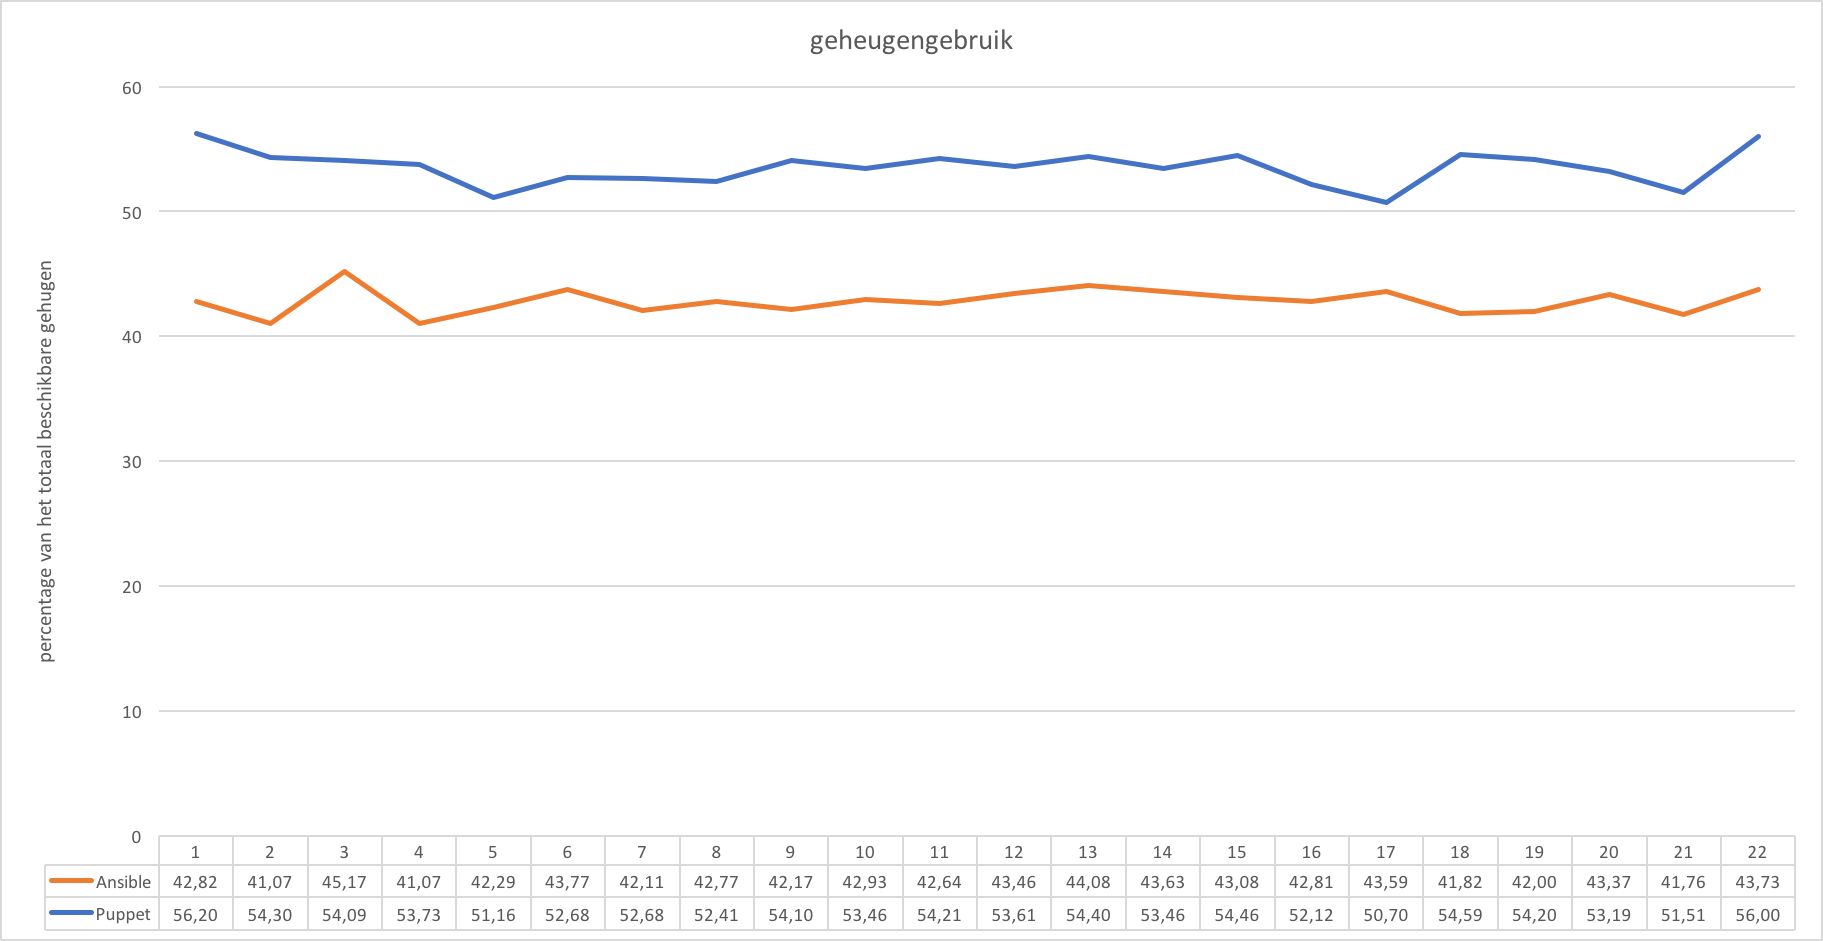
\includegraphics[width=\linewidth]{img/geheugengebruik}
 \caption{Verbruikt percentage van het RAM geheugen. Gemeten bij servers met elk 500 MB. }  
  \label{fig:geheugengebruik}
\end{figure}

%---------------------------------------------

\section{Schaalbaarheid}
\label{sec:schaalbaarheid}

\subsection{inleiding}
\label{sec:inleiding}
 Initieel was het de bedoeling dat het gedrag van de resources gemeten in \ref{sec:methodologie-technische-verschillen} gemeten zouden worden bij toenemende drukte door meer clients toe te voegen. Tijdens het opstellen van deze proef bleek dat dit geen bedrijfs-realistische situatie. Bij Ansible is het namelijk Ansible Tower die bepaald wanneer de clients ge\"updatet moeten worden. Bij Puppet valt dit onder de verantwoordelijkheid van de clients zelf. Bijgevolg is de kans klein dat in het geval van Puppet alle clients tegelijk een catalogus zouden aanvragen en hierdoor de Master zwaar belasten. Toch zijn er hier en daar zaken die de performantie ten goede komen. Zo blijft het downloaden van software de grootst bottleneck van een goede en snelle deploy. Heel wat verkeer moet het lokale netwerk verlaten om bestanden van een externe bron op te halen. Een oplossing hiervoor is om een lokale server op te stellen die een kopie bewaart van de (meest) gebruikte services. \autocite{AnsibleTuning}.
 
 \subsection{Tips om de performantie van Ansible te verbeteren}
 Standaard is Ansible geconfigureerd om 5 servers tegelijk te kunnen configureren. Dit aantal kan verhoogt worden naar de parameter \texttt{\gls{fork}s} naar 25 tot zelfs 100 te brengen. \newline
Ansible adviseerd verder ook om gebruik te maken van \texttt{with\_items} bij het installeren van meerdere packages. Dit komt omdat bij het gebruik van \texttt{with\_items}, Ansible deze packages zal combineren in \'e\'en transactie block dewelke de performantie ten goede komt. Zo zou het dus beter zijn om listing \ref{lst:yamltwotask} beter te structuren en te schrijven zoals in listing \ref{lst:yamlonetask}. \newline
Verder beschikt Ansible over een 'Pull-mode' waarbij elke server zelf instaat voor zijn configuratie. Elke server haalt de code op van een centraal punt en configureerd vervolgens zichzelf. Deze mannier van werken vereist wel een scriptje op elke server en doet denken aan de werking van Puppet. Een centraal management punt is in deze opstelling echter niet aanwezig en is dus af te raden voor grotere infrastructuren \autocite{AnsibleTuning} .

   \lstset{language=clean,caption={Installeer de vereiste onderdelen van PHP in twee delen},label={lst:yamltwotask}}
\begin{lstlisting}[frame=single]

- name: installeer PHP
  package:
    name: php
    state: present

- name: installeer php-mysql
  package:
    name: php-mysqli
    state: present
\end{lstlisting}

  \lstset{language=clean,caption={Installeer de vereiste onderdelen van PHP in \'e\'en keer},label={lst:yamlonetask}}
\begin{lstlisting}[frame=single]
- name: installeer PHP en bijhorende extensies
  package:
    name: {{ item }}
    state: present
  with_items:
    - php
    - php-mysqli
\end{lstlisting}

  
  
 \subsection{Tips om de performantie van Puppet te verbeteren}
 Puppet is door zijn mannier van werken van nature meer geloadbalanced dan Ansible, zie \ref{sec:inleiding}, toch zijn ook hier een paar zaken die de performantie ten goede komen. Het aantal aanvragen die Puppet tegelijk kan behandelen varieert van server tot server. Dit is standaard 'num-cpu's - 1' met een minimum van 1 en een maximum van vier. Het aantal gebruikte cpu's staat gelijk aan het aantal aanvragen die Puppet tegelijk kan behandelen. Wanneer er meer aanvragen zijn dan beschikbare CPU's zal het overschot aan aanvragen geblokkeerd worden totdat er een slot vrijkomt. Dit aantal kan handmatig verhoogd worden met behulp van de variabele \texttt{max-active-instances}. Wanneer deze naar bijvoorbeeld twee gebracht wordt zullen twee core's van de processor gebruikt worden, dit heeft tot gevolg dat er ook twee aanvragen tegelijk behandeld kunnen worden. \newline
 Een tweede zaak is het verhogen van de \texttt{max heap size} van JVM. Door dit te verhogen kan het JVM proces meer geheugen opvragen bij het besturingssysteem \autocite{PuppetTuning}.
 
 
 %---------------------------------------------------------------------------------------------------------------------------------------------------------------------------------------------------------------------------------------------------------------------------------------------------------------------------------------------------------------------------------------------------------------------------------------------------------------------------------------------------------------------------------------------------------------------------------------------------------------------------------------------------------------------------------------------------------------------------------------------------------------------------------------------------------------------------------------------------------------------------------------------------------------------------------------------------------------------------------------------------------------------------------------------------------------------------------------------------------%
\section{Wat is het verloop van een dergelijke transitperiode?}
\label{sec:methodologie-verloop-transit}



\begin{wrapfigure}{R}{0.4\textwidth}
\centering
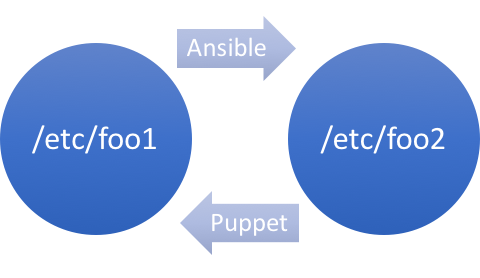
\includegraphics[width=0.4\textwidth]{img/vicieuzecirkel.PNG}
\caption{\label{fig:vicieuzecirkel}Vicieuze cirkel van twee \gls{CMT}'s hetzelfde bestand proberen te configureren.}
\end{wrapfigure}

Het is vanzelfsprekend dat de mannier van Ansible integreren afhankelijk is van bedrijf tot bedrijf. Toch is dit in het geval van de VRT vlot verlopen. Ansible en Puppet kunnen namelijk perfect naast elkaar in dezelfde infrastructuur bestaan. Dit is ideaal voor een geleidelijke overgang. E\'en en dezelfde server kan bovendien geconfigureerd worden door zowel Puppet als Ansible. Dit heeft als voordeel dat niet alle modules geschreven in Puppet onmiddellijk vertaald hoeven te worden. Enkele rollen kunnen geschreven zijn voor Ansible terwijl een ander deel nog onder de bevoegdheid van Puppet valt. Belangrijk hierbij is wel dat Puppet en Ansible verschillende configuraties behandelen. Wanneer beide \gls{CMT}'s eenzelfde configuratie uitvoeren kan er door subtiele verschillen een vicieuze cirkel ontstaan.\newline
Beeld u zich de situatie in zoals op figuur \ref{fig:vicieuzecirkel}. In ansible staat een bestand met een extra spatie, hier noemen we deze voor het gemak 'foo1'. Bij puppet staat deze extra spatie er niet, deze wordt 'foo2' genoemd. 
\begin{enumerate}
\item Puppet configureert de service met bestand foo2 en start deze op.
\item  Eventjes later stelt Ansible vast dat de configuratie niet meer overeenkomt met deze beschreven in het playbook. Hij wijzigt foo2 naar foo1 en herstart de service zodat aanpassingen doorgevoerd zouden worden.
\item  Op een later ogenblik zal Puppet dit waarnemen en het bestand terugdraaien naar foo1, opnieuw gevolgd door een gerstart van de gerelateerde service.
\end{enumerate}
Het is vanzelfsprekend dat dit zorgt voor onnodige aanpassingen met eventueel ongewenste of onverwachte gevolgen zoals het voortdurend herstarten van een service.\newline
Twee \gls{CMT}'s die dezelfde server op hetzelfde moment configureren zouden elkaar niet mogen hinderen. Ten hoogste duurt de configuratie iets langer omdat er een lock bestaat op de \gls{packagemanager}s waardoor de ene \gls{CMT} op de andere dient te wachten.



